\chapter{Metodologia} \label{cap3}

\section{Caracterização}

%\subsection*{Método de caracterização baseado na convolução não linear}
O método de caracterização foi baseado nos experimentos realizados por \cite{farina2001non} e utiliza o sinal de excitação de um sistema não linear descrito na subseção \ref{ident}. O método consiste em excitar o sistema em análise com um \textit{Swept Sine} e gravar a saída do sistema. Em seguida	realiza-se uma inversão temporal do sinal de excitação para realizar uma convolução com a resposta gravada do sistema em análise. Após essa convolução, obtém-se uma função constituída por respostas ao impulso seguidas conforme a figura \ref{fig:nlcir}.

\begin{figure}[!htb]
	\centering
	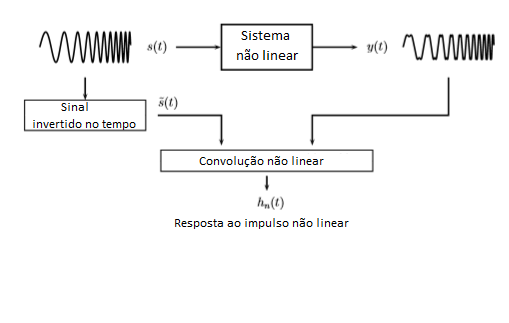
\includegraphics[width=0.9\linewidth]{figuras/NLCM}
	\caption{Diagrama de blocos do método baseado em convolução não linear. Autor: \cite{novakdissertation}}
	\label{fig:nlcm}
\end{figure}

A figura \ref{fig:nlcm} mostra os sinais $s(t)$ e $y(t)$ que são respectivamente, o sinal senoidal que varia exponencialmente na frequência e a saída do sistema em análise. O sinal $\overline{s}(t)$ é o sinal $s(t)$ invertido temporalmente. A convolução entre $y(t)$ e $\overline{s}(t)$ pode ser expressa por:
\begin{equation}
y(t) \ast \overline{s}(t) = \sum_{m=1}^{\infty}h_{m}(t + \Delta t_{m})
\label{kernel}
\end{equation}
Onde, $h_{m}$ é a resposta não linear ao impulso e $\Delta t_{m}$ é a diferença de tempo entre a primeira resposta impulsional e a em-ésima resposta do sistema, onde a primeira resposta define a parte linear do sistema em análise. Dessa forma é possível separar temporalmente cada resposta ao impulso, a partir do valor de $\Delta t_{m}$ como mostra a figura abaixo:

\begin{figure}
	\centering
	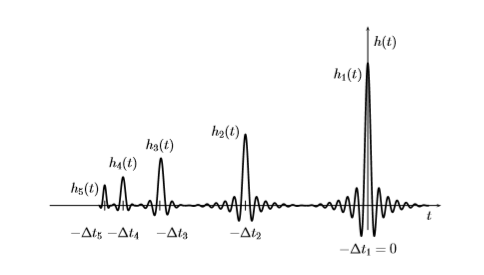
\includegraphics[width=0.6\linewidth]{figuras/NLCIR}
	\caption{Resposta ao impulso do sistema em análise. Autor: \cite{novakdissertation}}
	\label{fig:nlcir}
\end{figure}

Através do uso da Transformada de Fourier de cada resposta ao impulso é obtida a resposta frequencial de cada impulso como mostra a figura \ref{fig:nlcfr}
\begin{figure}
	\centering
	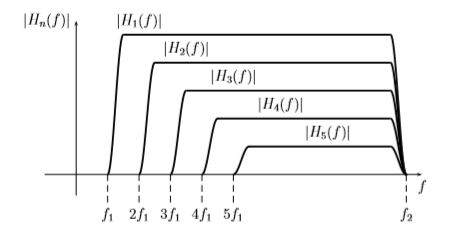
\includegraphics[width=0.6\linewidth]{figuras/NLCFR}
	\caption{Módulo da resposta frequencial dos impulsos. Autor:\cite{novakdissertation}}
	\label{fig:nlcfr}
\end{figure}

Na figura \ref{fig:nlcfr}, as frequências $f_{1}$ e $f_{2}$ são as frequências em que o sinal de excitação começa e termina, respectivamente.


O amplificador utilizado para a caracterização, mostrado na figura \ref{fig:Black}, é um \textit{Blackstar} HT-5 C, composto por uma válvula 12BH7 no pré amplificador e uma ECC83 na parte de amplificação de potência. Para evitar qualquer efeito memória proveniente da suspensão de um alto falante \cite{klippel2004dynamical} e possíveis modificações causadas devido ao uso de um microfone para gravar a saída do amplificador, todas as gravações realizadas foram feitas utilizando a saída do pré amplificador.

\begin{figure}
	\centering
	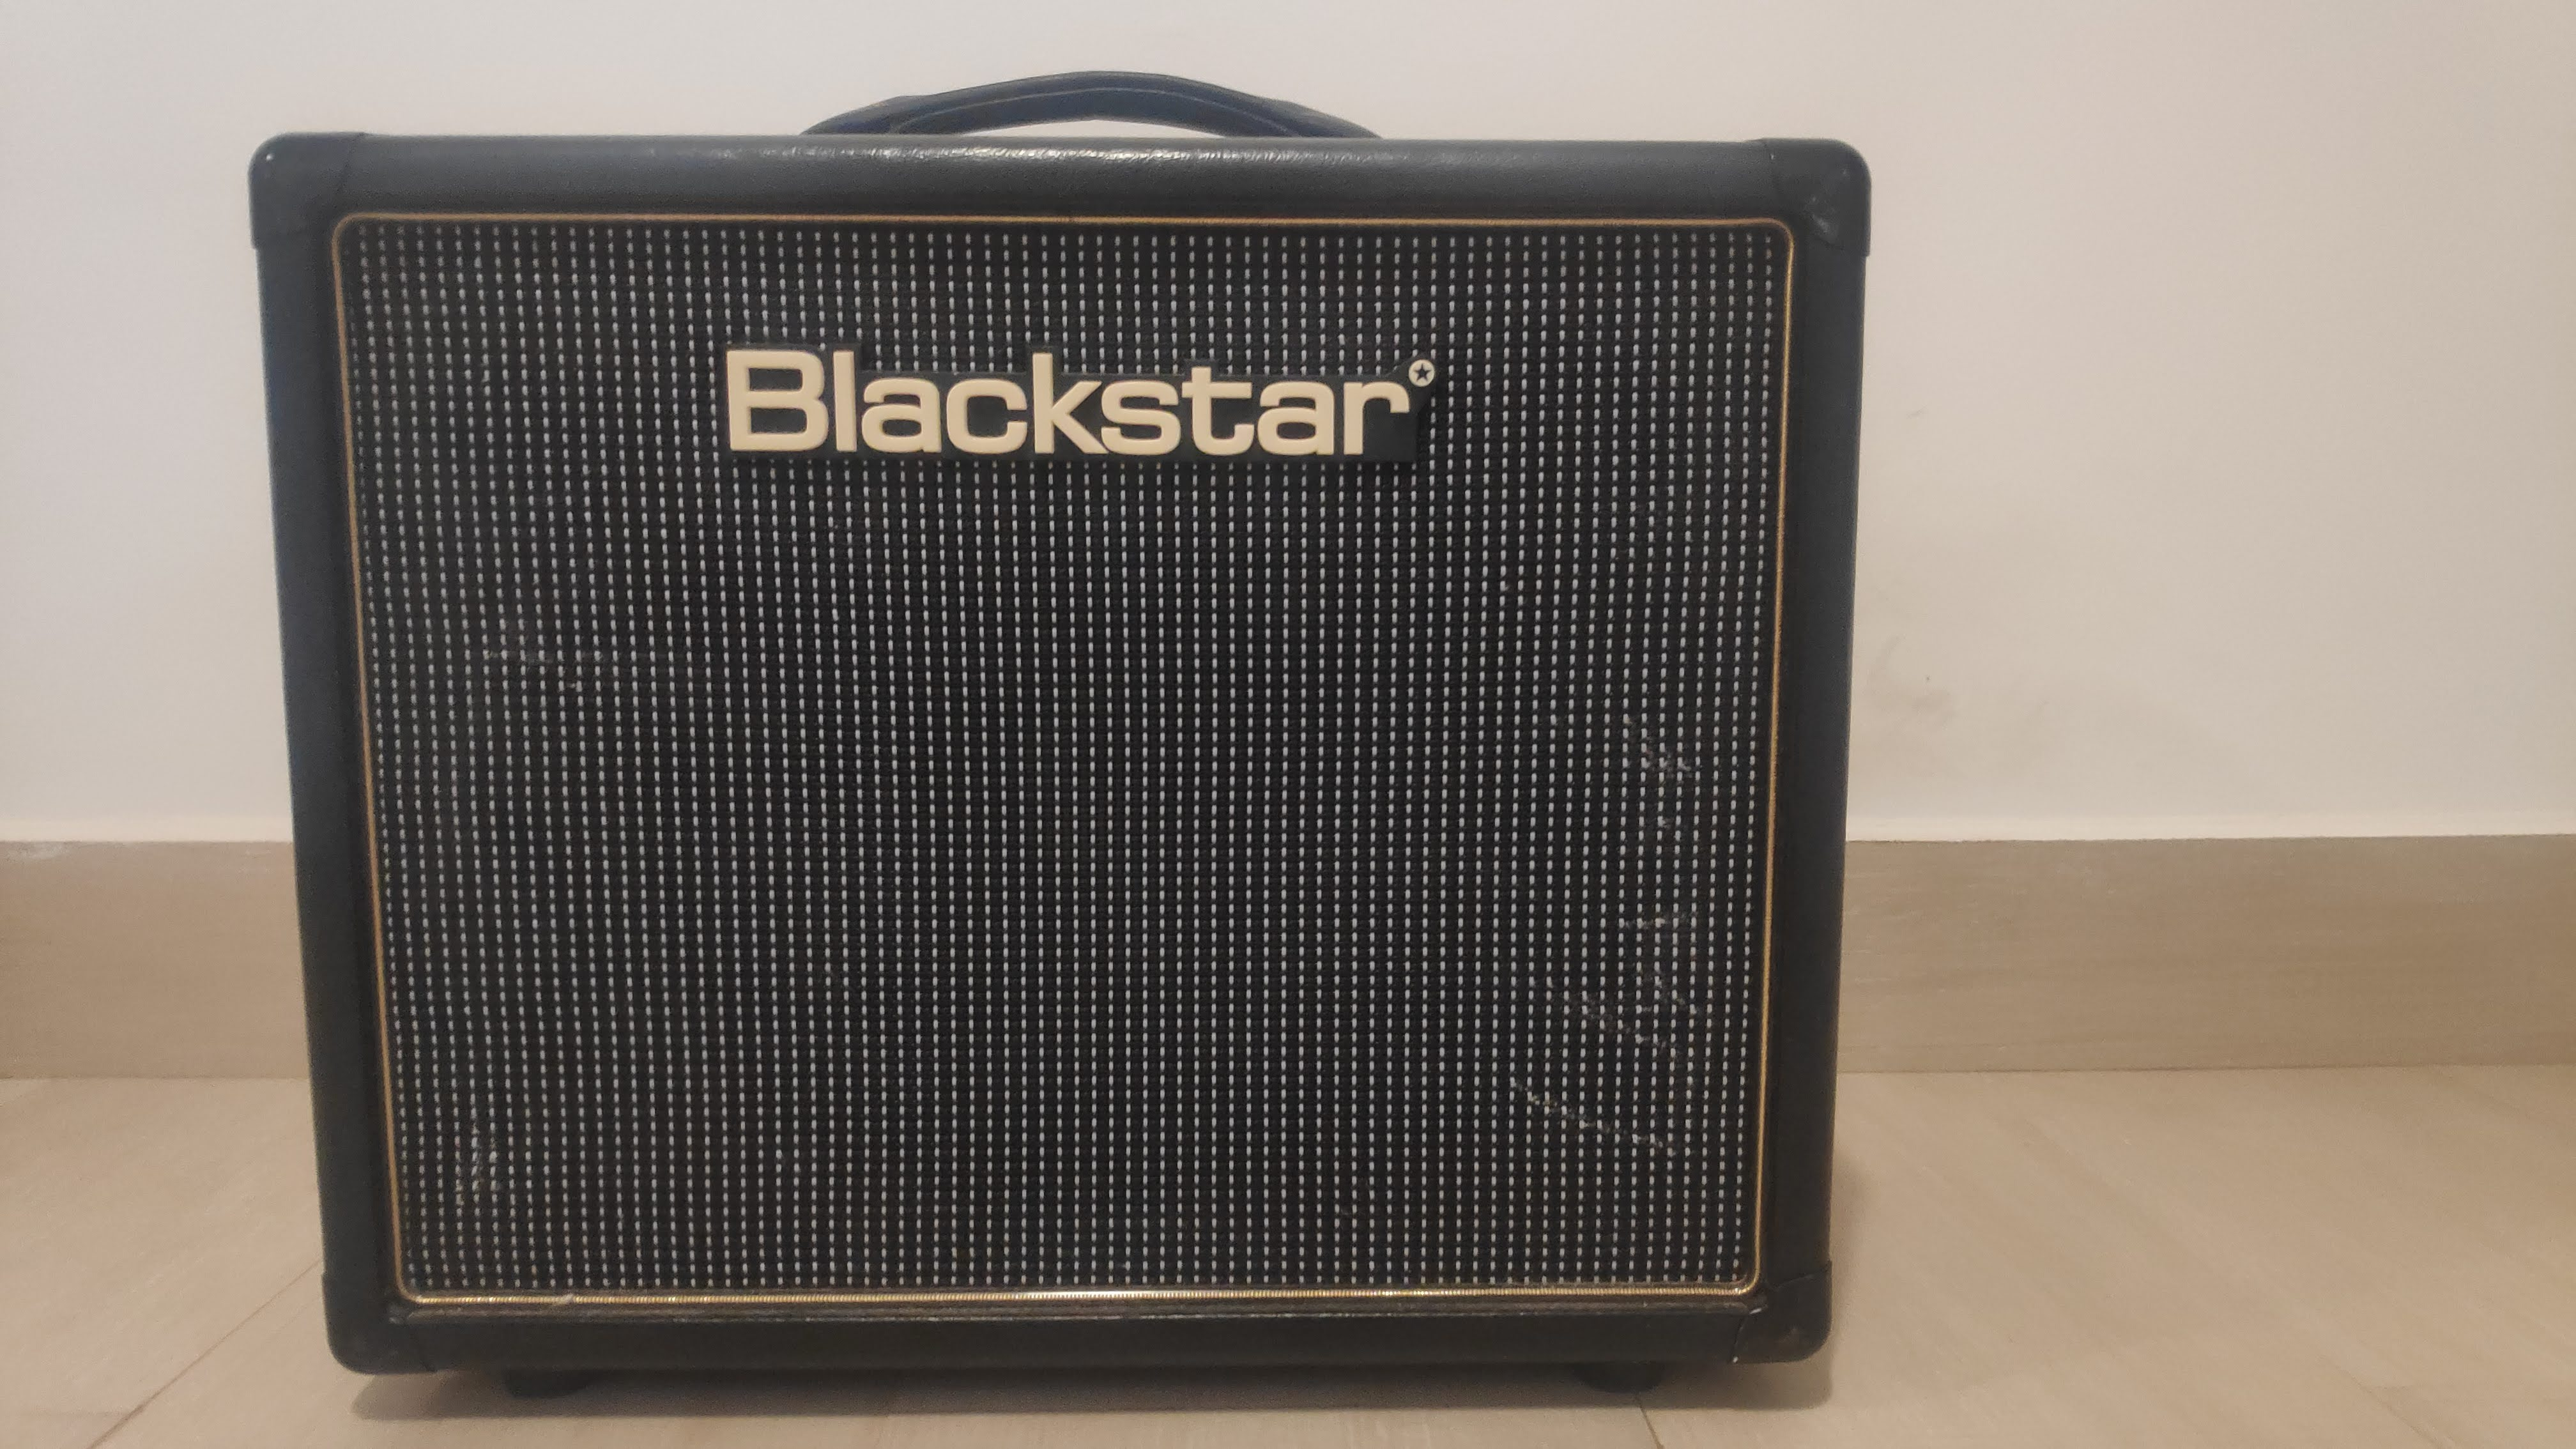
\includegraphics[width=0.7 \linewidth]{figuras/Blackstar1}
	\caption{Amplificador Blackstar HT-5 C}
	\label{fig:Black}
\end{figure}

A criação do sinal de teste foi feita segundo a equação \ref{sinal exponencial}, utilizando o programa Matlab para computar a função e gerar o arquivo de áudio em formato \textit{.wav}. O tempo de duração do sinal foi de 20 segundos, gerando 882000 amostras, devido a frequência de amostragem de 44,1 kHz e 16 bits de quantização para igualar as configurações usadas na interface de áudio USB utilizada durante o processo de gravação dos sinais.


O sinal exponencial então foi exportado em uma trilha mono, para o programa Audacity, que é um editor, gravador e reprodutor de áudio e configurada para enviar o sinal para a saída da interface. Utilizando a interface de áudio M-audio \textit{Fast Track Pro}, conectou-se a saída do pré amplificador presente no \textit{Blackstar} à entrada de áudio da interface, através de um cabo P10. A saída da interface, por onde o sinal exponencial é enviado do computador, foi conectada à entrada de instrumentos do amplificador. No software Audacity, foi criada uma segunda trilha de áudio armada para gravar o sinal na entrada da interface. 


A figura \ref{fig:diag} mostra como foram feitas as conexões entre computador, interface e amplificador.
\begin{figure}
	\centering
	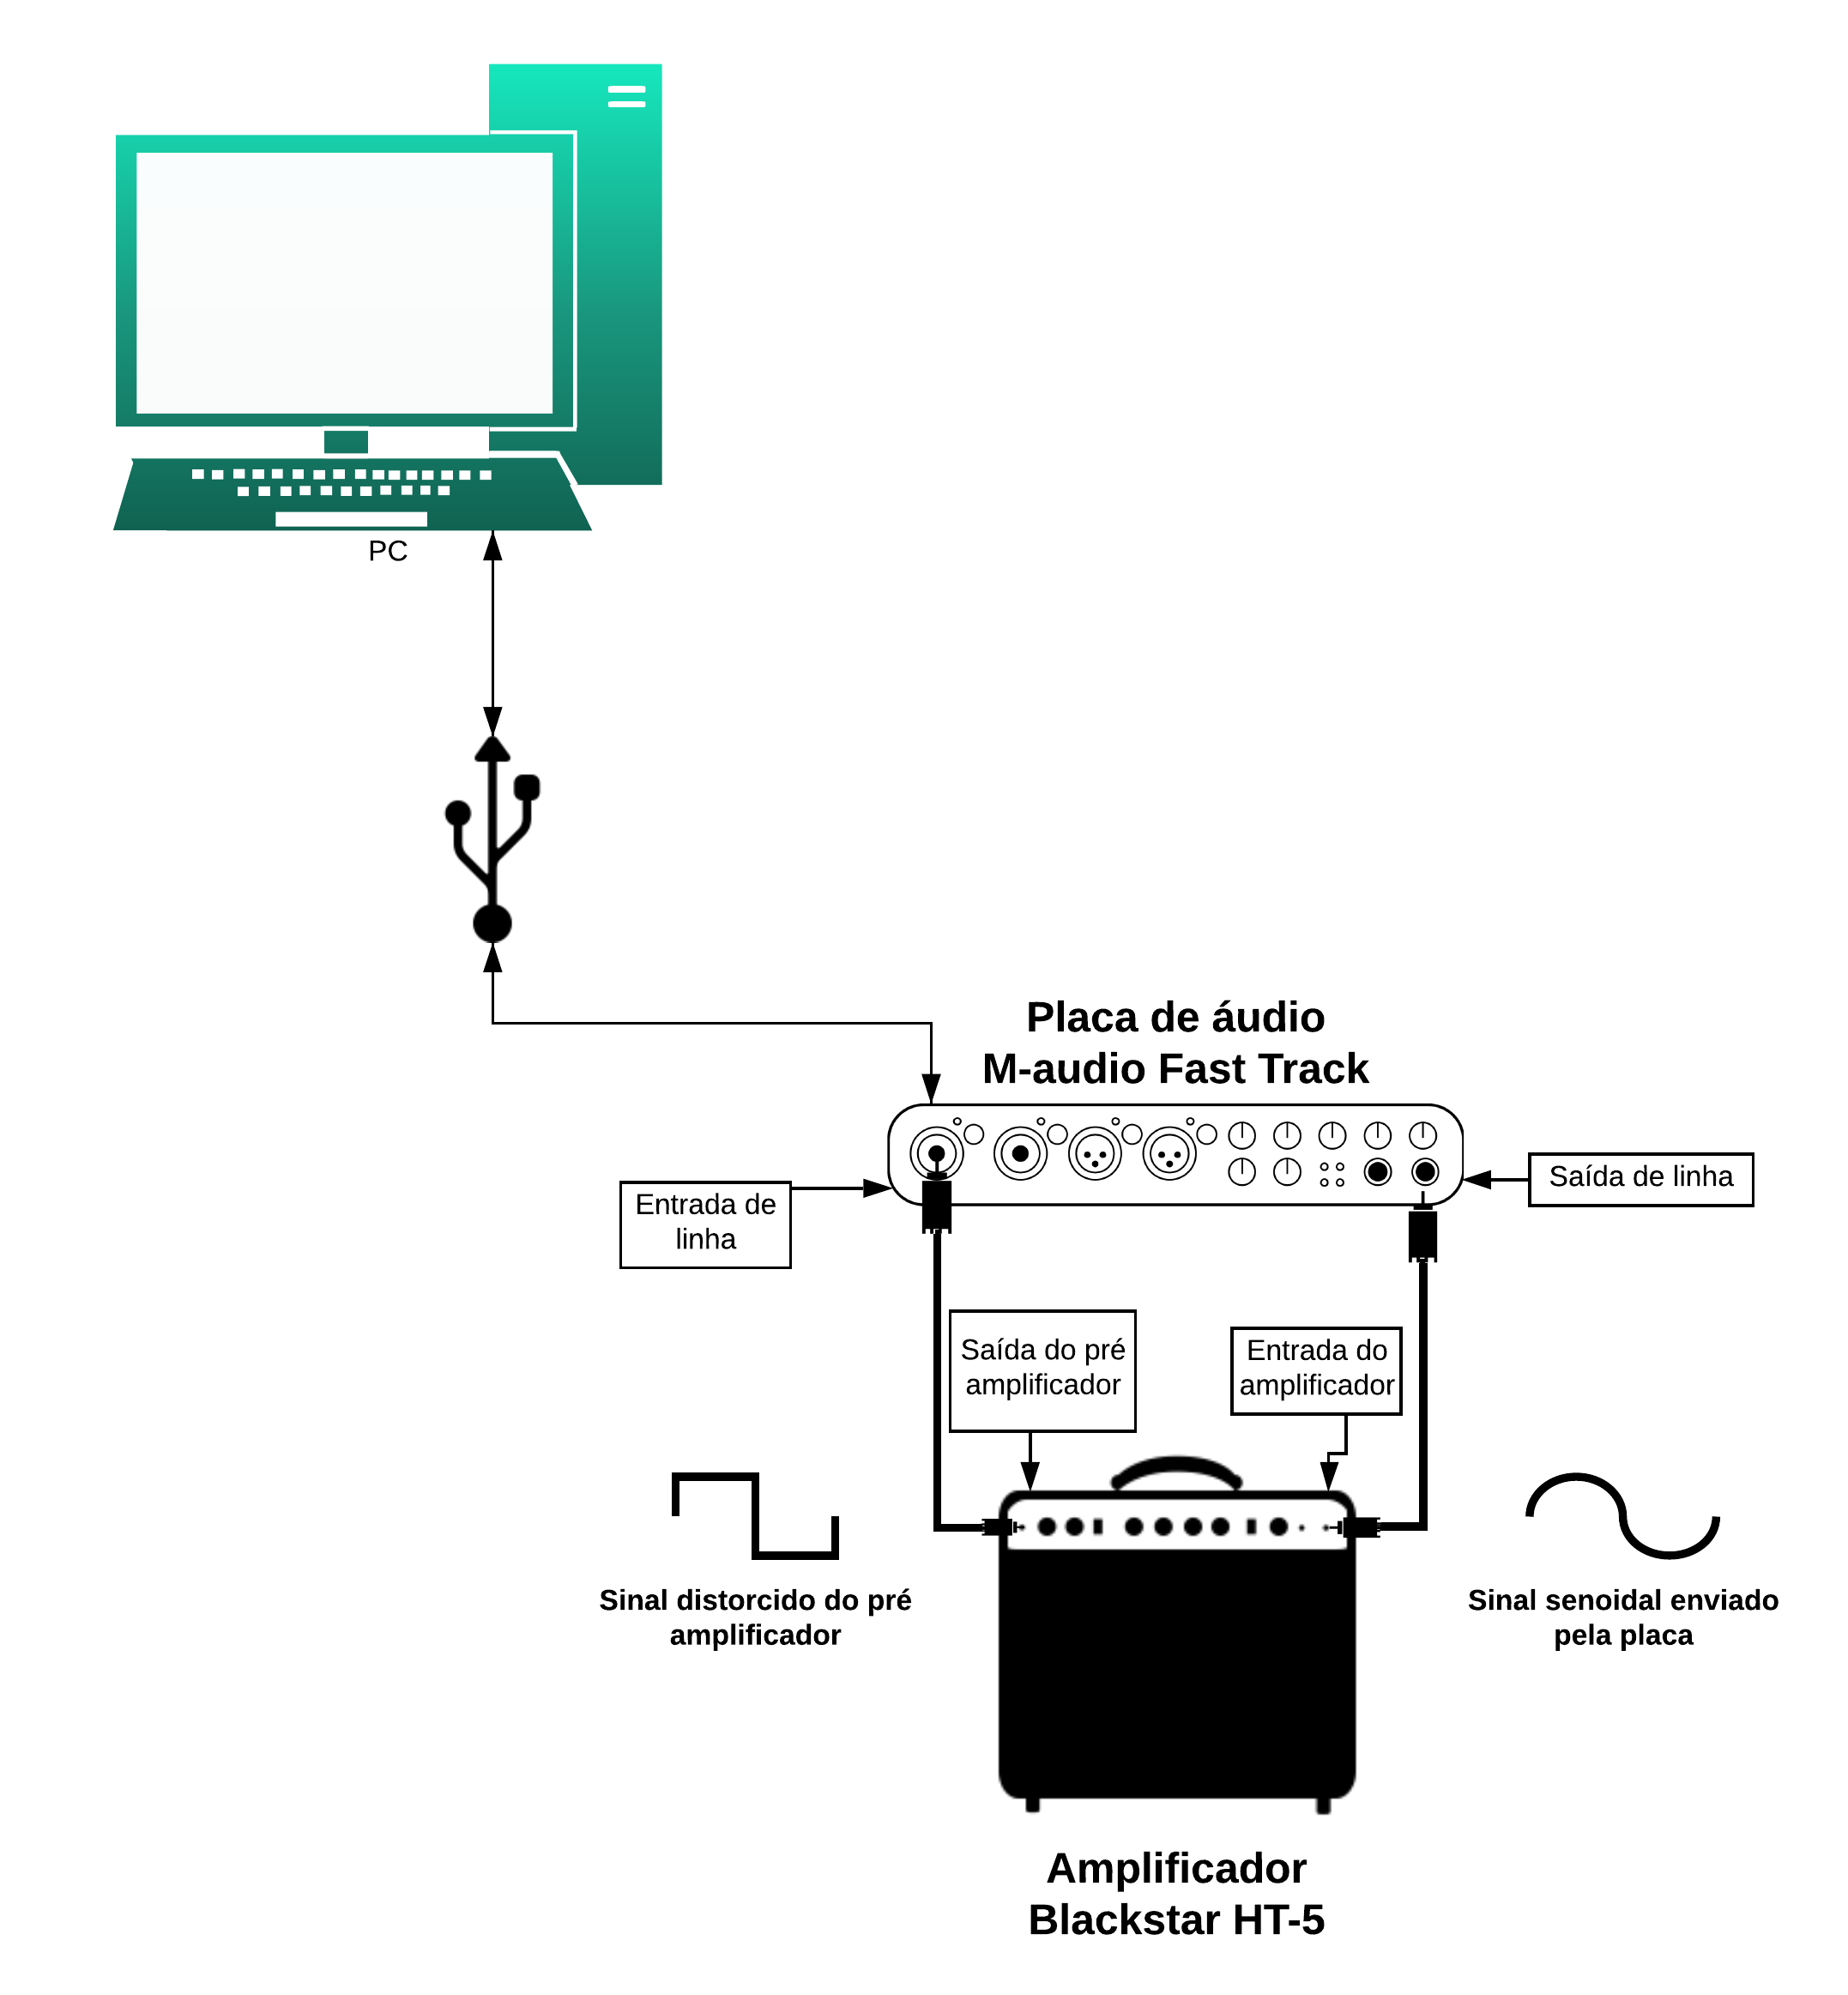
\includegraphics[width=0.7\linewidth]{figuras/diag}
	\caption{Diagrama de conexão do sistema de caracterização}
	\label{fig:diag}
\end{figure}

Após a gravação do sinal exponencial na saída do pré amplificador, o arquivo contendo as informações foi exportado para o Matlab onde foi processado e convoluído com o sinal exponencial invertido para obtenção dos \kernels, como mostra a figura \ref{fig:nlcm}. Seguindo a extração dos \kernels, separou-se cada impulso obtido, exemplificado na figura \ref{fig:nlcfr}, para a construção do modelo de \textit{Hammerstein} do amplificador, de acordo com a figura \ref{fig:hammer}


\begin{figure}
	\centering
	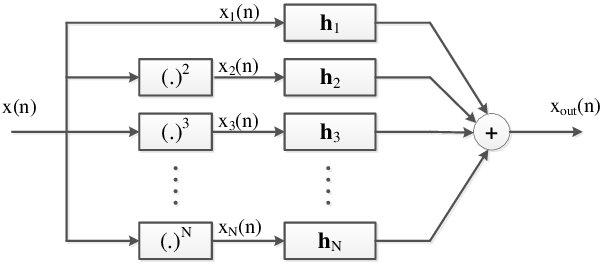
\includegraphics[width=0.5\linewidth]{figuras/hammer}
	\caption{Modelo de \textit{Hammerstein}. Retirado de: \cite{inproceedings}}
	\label{fig:hammer}
\end{figure}

\pagebreak
A ordem do sistema, ou seja, a quantidade de \kernels utilizados para construir o modelo de \textit{Hammerstein}, foi ajustada para utilizar 11 \kernels. A escolha de 11 núcleos foi devido a quantidade de respostas ao impulso que foram separadas sem que houvesse interferência de um impulso adjacente, a figura \ref{fig:nlcfr} exemplifica como a diferença temporal $\Delta t$ entre os impulsos se trona estreita com o aumento do tempo . A saída do sistema então foi obtida, com a convolução de 11 sinais, cada um elevado a um expoente, cujo valor máximo é determinado pela ordem do sistema, com um núcleo associado a cada expoente. Esses sinais são somados resultando em um único sinal de áudio que representa a saída final do modelo caracterizado. 

A figura \ref{fig:diagramamatlab} exemplifica o funcionamento do algorítimo criado para a simulação do amplificador caracterizado. Primeiramente carrega-se a saída do gravada do amplificador a ser modelado (variável y), utilizando a transformada de Fourier é obtido a resposta frequencial do amplificador ao sinal senoidal exponencial (variável Y). O sinal exponencial invertido no tempo é gerado assim como sua resposta frequencial (variável S). De posse da resposta frequencial da saída do amplificador e do sinal senoidal exponencial invertido no tempo, é possível obter os núcleos da série de volterra multiplicando as duas respostas frequenciais. A separação de cada resposta impulsional é feita com a criação de um vetor, nomeado dt, onde cada posição do vetor é a posição exata de cada $\Delta t$ conforme a figura \ref{fig:nlcfr}. A aplicação do modelo de \textit{Hammerstein} é feita após a individualização de cada resposta impulsional, onde é carregado qualquer sinal que se deseja obter a saída e esse sinal então é normalizado para que a sua amplitude máxima não ultrapasse o limite máximo que o Matlab opera sem distorcer o sinal. Este sinal é então elevado até a quantidade de núcleos que se deseja utilizar, ou seja até o valor da ordem escolhida para o sistema (Variável N). São obtidos então N sinais elevados, cada um desses sinais é então convoluído com uma resposta impulsional. A saída de cada convolução é somada gerando um único sinal que é, por fim, a saída do sistema modelado.


\begin{figure}[!htb]

	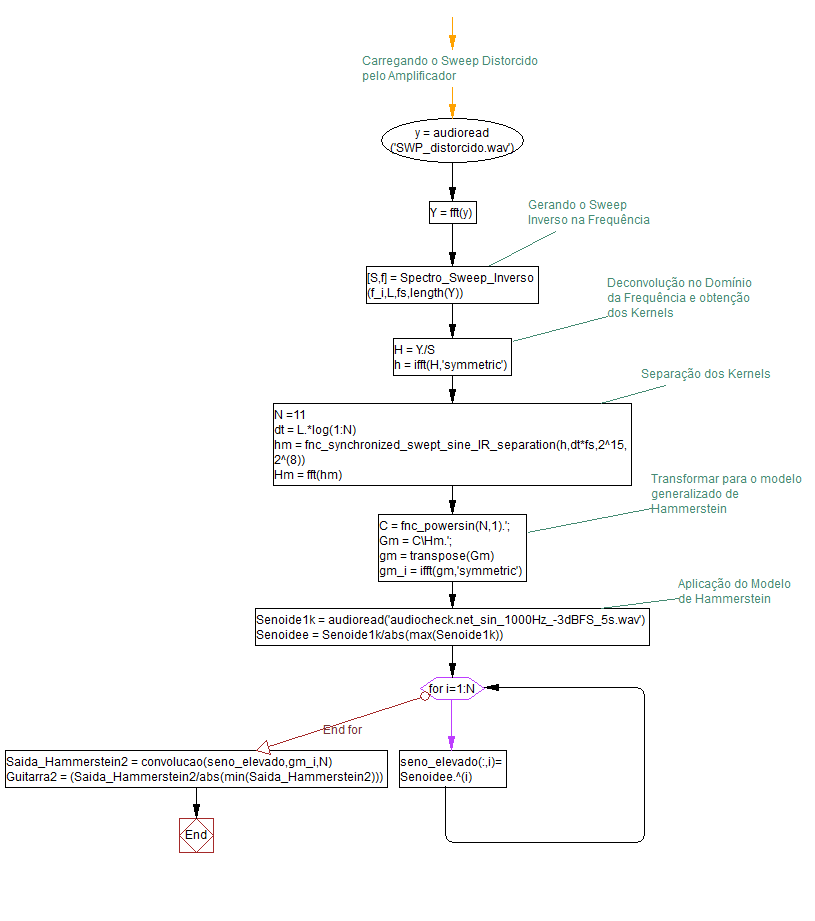
\includegraphics[width=1.0\linewidth]{figuras/Diagrama_Matlab}
	\caption{Fluxograma do programa desenvolvido}
	\label{fig:diagramamatlab}
\end{figure}
